%
%     hw1_bbordwell.tex
%     Baylee Bordwell (baylee.bordwell@colorado.edu)
%     Based on the template by Benjamin Brown (bpbrown@colorado.edu)
%     Aug 27, 2014
%
%     Problem set 1 for ASTR/ATOC 5540, Mathematical Methods, taught at
%     University of Colorado, Boulder, Fall 2014.
%
%

\documentclass[12pt, preprint]{aastex}
% formatting based on 2014 NASA ATP proposal with Jeff Oishi

%%%%%%begin preamble
\usepackage[hmargin=1in, vmargin=1in]{geometry} % Margins
\usepackage{hyperref}
\usepackage{url}
\usepackage{times}
\usepackage{natbib}
\usepackage{graphicx}
\usepackage{amsmath}
\usepackage{amsfonts}
\usepackage{amssymb}
\usepackage{pdfpages}
\usepackage{import}
% for code import
\usepackage{listings}
\usepackage{color}


\hypersetup{
     colorlinks   = true,
     citecolor     = gray,
     urlcolor       = blue
}

%% headers
\usepackage{fancyhdr}
\pagestyle{fancy}
\lhead{ASTR/ATOC 5540}
\chead{}
\rhead{name: Baylee Bordwell}
\lfoot{Problem Set 1}
\cfoot{\thepage}
\rfoot{Fall 2014}
% no hline under header
\renewcommand{\headrulewidth}{0pt}

\newcommand{\sol}{\ensuremath{\odot}}
\newcommand{\dedalus}{\href{http://dedalus-project.org}{Dedalus}}

% make lists compact
\usepackage{enumitem}
%\setlist{nosep}

%%%%%%end preamble


\begin{document}

\section*{Problem Set 1}

\begin{enumerate}
  \item In final plot.

  \item 
    The FD-1 approximation first displays larger, sporadic error which decreases until about $\Delta x = 10^{-8.5}$, when the error in the approximation begins to grow linearly. The smallest error in $f^\prime(x0)$ is about $10^{-9}$, and it occurs at approximately $\Delta x = 10^{-8.5}$ . This is the effect of the roundoff error diminishing as the dominant source of error in the estimate, and the discretionary error taking over, as can be seen when the discretionary error is added into the plot.

  \item 
    \begin{equation} \nonumber
      f(x0+\Delta x) = f(x0)+
      \Delta xf^{\prime}(x0)+  
      \frac{\Delta x^2}{2}f^{\prime\prime}(x0)+\cdots  
    \end{equation}
    \begin{equation} \nonumber
      f^{\prime}(x0) =   \frac{f(x0+\Delta x)-f(x0)}{\Delta x}+
      \frac{\Delta x}{2}f^{\prime\prime}(x0)+\cdots  
    \end{equation}
    Discretionary error $D$ is approximated as the first neglected term, 
    $D \approx \frac{\Delta x}{2}f^{\prime\prime}(x0)$.


   \item $f(x0+\Delta x) $ can be seen above, 
     \begin{equation} \nonumber
       f(x-\Delta x) = f(x0)-
       \Delta xf^\prime(x0)+  
       \frac{\Delta x^2}{2}f^{\prime\prime}(x0)+\cdots  
     \end{equation}
     \begin{equation} \nonumber
       f^\prime_{FD-2}(x0) = \frac{f(x0+\Delta x)-f(x0-\Delta x)}{2\Delta x}
     \end{equation}
     \begin{equation} \nonumber
       = \frac{1}{2\Delta x}(
       f(x0)+\Delta xf^\prime(x0)+
       \frac{\Delta x^2}{2}f^{\prime\prime}(x0)+\cdots  
       -(f(x0)-\Delta xf^\prime(x0)+
       \frac{\Delta x^2}{2}f^{\prime\prime}(x0)+\cdots))
     \end{equation}
     \begin{equation} \nonumber
       = f^\prime(x0)+ \frac{\Delta x^2}{6}f^{\prime\prime\prime}(x0)+ \cdots
     \end{equation}
     FD-2 is special in comparison to FD-1 because it removes all terms even in powers of $\Delta x$ from the Taylor expansion, resulting in a smaller discretionary error, $D \approx \frac{\Delta x^2}{6}f^{\prime\prime\prime}(x0)$


    \item The FD-2 approximation behaves similarly to the FD-1, but with a consistently lower absolute error.


    \item  FD-1 is a first order approximation because we lose all terms after the first derivative in a Taylor expansion of $f$, while FD-2 is a second order approximation because we lose all terms after the second derivative in a Taylor expansion of $f$. If we want the lowest error at the lowest computational cost, FD-2 is better to use because we can use a larger $\Delta x$ and achive a lower error than with FD-1.


\end{enumerate}
\begin{figure}
  \centering
  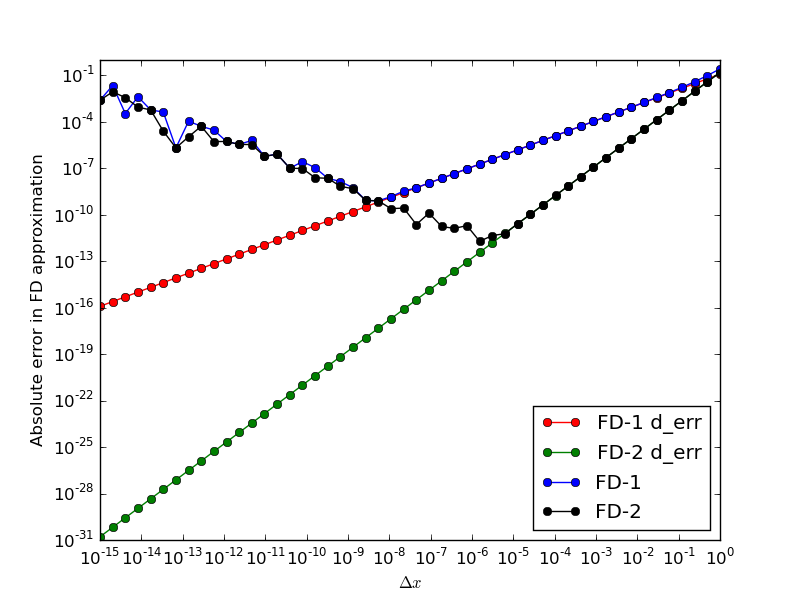
\includegraphics[width=\textwidth]{hw1_fig1.png}
\end{figure}


%
%     hw1_code.tex
%     Benjamin Brown (bpbrown@colorado.edu)
%     Aug 27, 2014
%
%     Problemset 1 for ASTR/ATOC 5540, Mathematical Methods, taught at
%     University of Colorado, Boulder, Fall 2014.
%
%     Python code importing block.
%


\definecolor{codegreen}{rgb}{0,0.6,0}
\definecolor{codegray}{rgb}{0.5,0.5,0.5}
\definecolor{codepurple}{rgb}{0.58,0,0.82}
\definecolor{backcolour}{rgb}{0.95,0.95,0.92}
 
\lstdefinestyle{mystyle}{
    backgroundcolor=\color{backcolour},   
    commentstyle=\color{codegreen},
    keywordstyle=\color{magenta},
    numberstyle=\tiny\color{codegray},
    stringstyle=\color{codepurple},
    basicstyle=\footnotesize,
    breakatwhitespace=false,         
    breaklines=true,                 
    captionpos=b,                    
    keepspaces=true,                 
    numbers=left,                    
    numbersep=5pt,                  
    showspaces=false,                
    showstringspaces=false,
    showtabs=false,                  
    tabsize=2
}

\lstset{style=mystyle}


\lstinputlisting[language=Python]{hw1_bbordwell.py}


\end{document}
